% begin module arc-length-intro
\begin{frame}
\frametitle{Arc Length}
\begin{center}

%\psset{xunit=1cm, yunit=1cm}
%\begin{pspicture}(-1.500000, -5)(1.500000,5) 
%\psframe*[linecolor=white](-1.500000,-5)(1.500000,5) 
%\tiny 
%\psaxesStandard{-1.000000}{-4.5}{1.000000}{4.5}
%\psplot[linecolor=\psColorGraph, plotpoints=1000]{-1.000000}{1.000000}{1 x 2 exp -1 mul add sqrt -1 mul }
%Function formula: \sqrt{- x^{2}+1} 
%\psplot[linecolor=\psColorGraph, plotpoints=1000]{-1.000000}{1.000000}{1 x 2 exp -1 mul add sqrt }
%\end{pspicture} 


\ \only<-2>{%
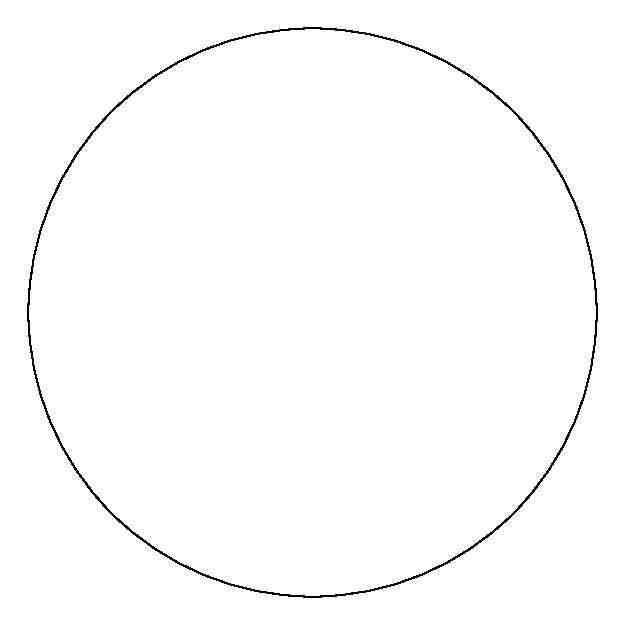
\includegraphics[height=4cm]{arc-length/pictures/09-01-circlea.pdf}%
}%
\only<handout:0| 3>{%
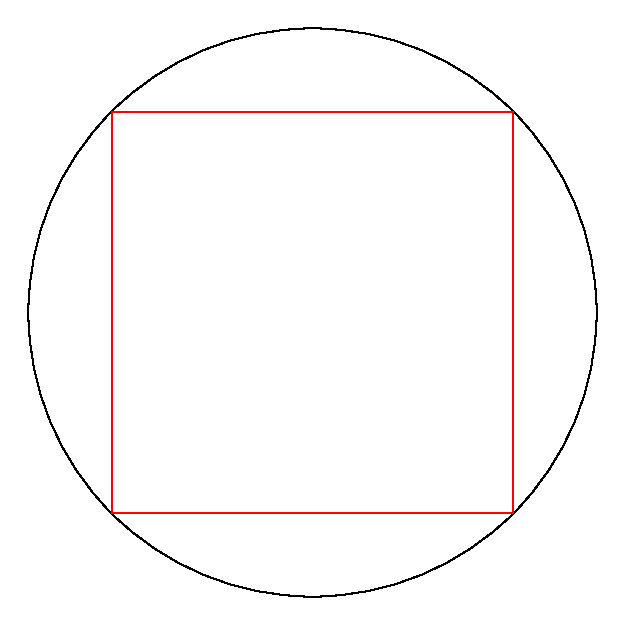
\includegraphics[height=4cm]{arc-length/pictures/09-01-circleb.pdf}%
}%
\only<handout:0| 4>{%
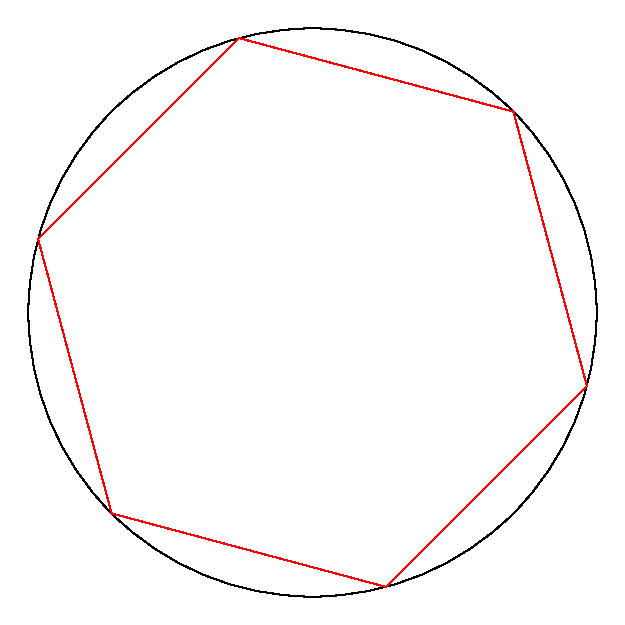
\includegraphics[height=4cm]{arc-length/pictures/09-01-circlec.pdf}%
}%
\only<handout:0| 5>{%
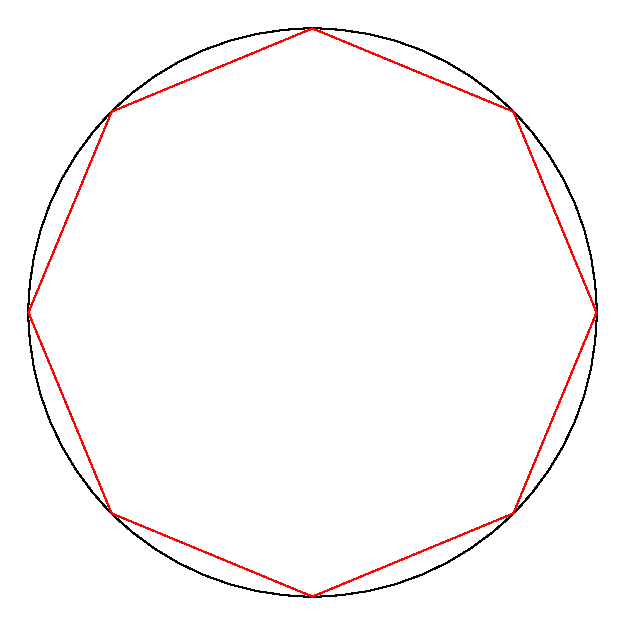
\includegraphics[height=4cm]{arc-length/pictures/09-01-circled.pdf}%
}%
\only<handout:0| 6>{%
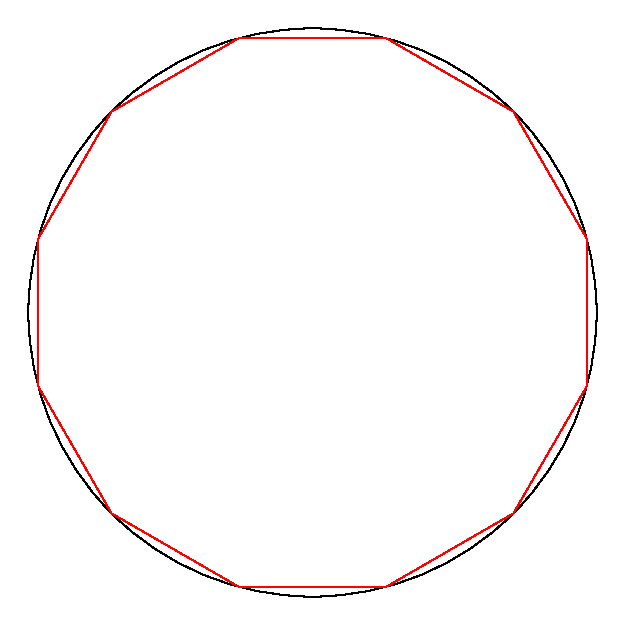
\includegraphics[height=4cm]{arc-length/pictures/09-01-circlee.pdf}%
}%
\only<handout:0| 7->{%
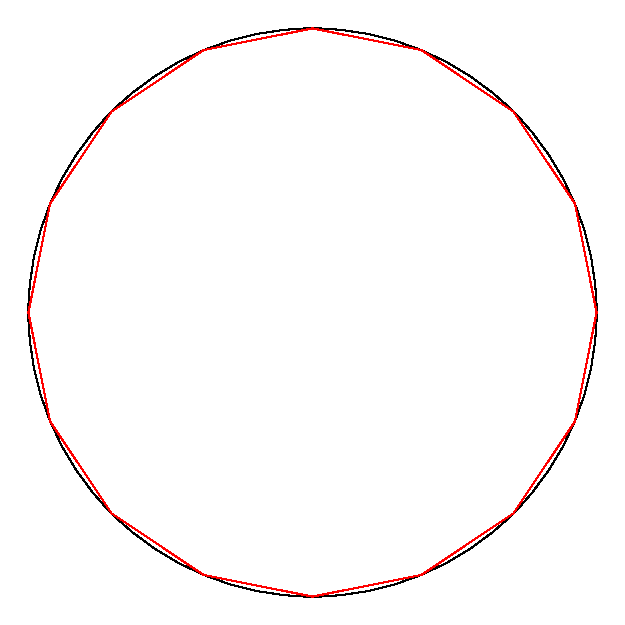
\includegraphics[height=4cm]{arc-length/pictures/09-01-circlef.pdf}%
}%
\end{center}
\begin{itemize}
\item  What do we mean by the length of a curve?
\item<2->  The length of a polygon is easy to compute: add up the length of the line segments that form the polygon.
\item<3->  If the curve is a circle, approximate it by a polygon.
\item<4->  Then take the limit as the number of segments of the polygon goes to $\infty$.
\end{itemize}
\end{frame}
% end module arc-length-intro
